\documentclass[a4paper,12pt]{report}

\usepackage[utf8]{inputenc}
\usepackage[russian]{babel}
\inputencoding{utf8}
\usepackage{graphicx}
\usepackage{caption}
\usepackage{subcaption}
\usepackage{float}
\usepackage{setspace}
\usepackage{eurosym}
\usepackage{hyperref}
\graphicspath{{Images/}}

\makeatletter
\renewcommand\chapter{\par%
\thispagestyle{plain}%
\global\@topnum\z@
\@afterindentfalse
\secdef\@chapter\@schapter}
\makeatother

\usepackage{geometry} % Меняем поля страницы
\geometry{left=2cm}% левое поле
\geometry{right=1.5cm}% правое поле
\geometry{top=3cm}% верхнее поле
\geometry{bottom=2cm}% нижнее поле

\renewcommand{\baselinestretch}{1.5}

\begin{document}

\begin{titlepage}
\begin{center}
{\large САНКТ-ПЕТЕРБУРГСКИЙ ГОСУДАРСТВЕННЫЙ УНИВЕРСИТЕТ \\[6mm] Кафедра Aстрономии }\\
\vspace{2cm}
{\Large \bf Мазурин Константин Эдуардович } \\
\vspace{2cm}
{\LARGE \bf Построение сети базовых ГНСС-станций } \\
\vspace{2cm}
{\large \bf Дипломная работа } \\[12mm]
\end{center}

\begin{flushright}
{\setstretch{1.0} \large Допущен к защите. \\[4mm]
{\it Заведующий кафедрой:} \\
д.ф.-м.н., профессор {\Large Витязев В.В.}\\ [4mm]
{\it Научный руководитель:} \\
к.ф.-м.н., доцент {\Large Петров С.Д.}\\ [4mm]
{\it Рецензент:} \\
\\ }
\end{flushright}
\vspace{5cm}
\begin{center}
{\large Санкт-Петербург \\[5mm] 2016}
\end{center}
\end{titlepage}

\begin{titlepage}
\begin{center}
{\large SAINT-PETERSBURG STATE UNIVERSITY \\[6mm] Chair of Astronomy }\\
\vspace{2cm}
{\Large \bf Mazurin Konstantin } \\
\vspace{2cm}
{\LARGE \bf Development of the GNSS reference stations network } \\
\vspace{2cm}
{\large \bf Graduation Thesis } \\[12mm]
\end{center}

\begin{flushright}
{\setstretch{1.0} \large Admitted for defence. \\[4mm]
{\it Head of the chair:} \\
Dr.Sci. (Phys.-Math.), Prof. {\Large Vityazev V.V.}\\ [4mm]
{\it Scientific supervisor:} \\
Cand.Sci (Phys.-Math.), Assoc.Prof. {\Large Petrov S.D.}\\ [4mm]
{\it Reviewer:} \\
\\ }
\end{flushright}
\vspace{5cm}
\begin{center}
{\large Saint-Petersburg \\[5mm] 2016}
\end{center}
\end{titlepage}

{\large\tableofcontents}
\newpage

\large
\chapter*{Введение}
\addcontentsline{toc}{chapter}{Введение}
\par ГНСС, или Глобальные Навигационные Системы Станций, - это технология, получившая очень широкое распространение в последнее десятилетие.
Системы GPS, ГЛОНАСС, а также быстро набирающие обороты Galileo (Европейский Союз) и BeiDou (Китай), постепенно становятся неотъемлемым
атрибутом повседневной жизни современного человека, хотя задумывались первые две исключительно в военных целях. Сейчас ГНСС используются
в различных отраслях жизнедеятельности человека. Военная и гражданская навигация, астрономия, геодинамика, сельское хозяйство, 
киноиндустрия - это лишь малая часть обширного списка. \par
В общем случае ГНСС состоит из нескольких основных компонентов: созвездия космических спутников, наземного сегмента, отвечающего за 
контроль и управление системой спутников, и аппаратуры потребителя ("спутниковых навигаторов"). Базовый принцип работы ГНСС достаточно 
прост. Для того, чтобы узнать свое местоположение, пользователь принимает сигналы, испускаемые спутниками. Сигнал от каждого спутника 
содержит его точные координаты (за это отвечает наземный сегмент) и временную отметку испускания этого сигнала в системе часов спутника. 
По времени распространения сигнала от спутника к приемнику вычисляется расстояние между ними. Получив сигналы от трех спутников 
(в реальности созвездия устроены так, что в каждый момент в любой точке планеты можно увидеть более 4 спутников), при помощи несложных 
вычислений приемник получает свое положение в пространстве. \par
Разумеется, как и любое измерение, подобный метод подвержен влиянию ошибок. Основные помехи вносит атмосфера, замедляя идущий из 
космоса сигнал. К другим источникам помех можно отнести переотражение сигнала от различных объектов, неточное знание эфемерид спутников 
или поправки часов приемника. Иногда влияние этих ошибок может существенно исказить конечный результат. И если во многих повседневных
задачах можно обойтись средней точностью измерения положения, составляющей $\approx$10м, то в ряде научных и военных задач такой точности 
явно недостаточно. Для подобных целей существуют более точные методы, позволяющие повысить точность до $\approx$1см, - DGNSS. 
Эти методы не ограничиваются использованием единичных ГНСС-приемников. Они используют т.н. сети базовых станций. В роли базовой станции
(base station) выступает приемник, установленный в месте с хорошо известными заранее координатами. Он проводит наблюдения спутников и 
вычисляет свое местоположение. По разнице вычисленных и известных заранее координат находятся поправки, которые в данном месте в данный 
момент влияют на результаты. После этого любой приемник, находящийся недалеко от данной базовой станции, - т.н. ровер (от англ. rover) - 
может получить поправки и, применив их к собственным измерениям, уточнить свои результаты. Важным допущением в данном методе является то, 
что поправки можно считать одинаковыми в пределах некоторой области вокруг базовой станции - порядка нескольких десятков километров. \par
На данный момент существует определенное количество подобных сетей, как международных, так и российских. Среди международных можно 
выделить IGS (International GNSS Service) - крупнейшую сеть из почти 500 станций, расположенных по всему миру, и EUREF Permanent GNSS 
Network - обширную Европейскую сеть, в которую входит чуть больше 300 станций. К большому сожалению, доля российских станций в обеих 
сетях мала: в IGS их насчитывается около 20, а в EUREF - всего 4. В итоге жители России, за небольшим исключением, не имеют возможности 
пользоваться этими инструментами. В России также есть свои сети базовых станций. Наиболее известные из них: СмартНет, GeoSpider и Hive GNSS.
Они обеспечивают хорошее покрытие Европейской части России (одна только Hive имеет в своем распоряжении около 400 станций), но у всех 
них есть один существенный недостаток - доступ к их данным платный. Помимо этого существует еще ряд проблем, связанных с этими сетями. 
К ним можно отнести закрытость исходных кодов ПО; невозможность автоматической загрузки данных; неравномерность расположения базовых 
станций - большая часть расположена вблизи Москвы и Санкт-Петербурга. \par
Целью данной выпускной квалификационной работы было создание прототипа подобной системы для отладки и дальнейшего применения в ряде
научных задач. Коренным отличием проектируемой сети от упомянутых выше является ее бесплатность и доступность для любых пользователей. 
Также программное обеспечение будет полностью открытым, что позволит другим пользователям без особых проблем улучшать и модернизировать 
систему под свои нужды.
В нашем распоряжении уже имеется некоторое количество ГНСС-приемников, расположенных на территории Санкт-Петербурга и Ленинградской
области, которые могут быть использованы в качестве базовых станций. Стояла задача объединить их в сеть, т.е. настроить сбор и передачу 
ГНСС данных по протоколу NTRIP (Networked Transport of RTCM via Internet Protocol), протестировать ее работу и попытаться воспользоваться 
ею для исследования геодинамики сопряжения Балтийского щита с Восточно-Европейской платформой - задачи, которой уже несколько лет 
занимаются сотрудники кафедры астрономии. В будущем мы планируем расширять сеть за счет подключения к ней новых базовых станций. \par
На данный момент мною были изучены возможности реализации данного проекта, был настроен сервер 
для приема, накопления и последующего распространения поправок, а также была написана программа, организующая сбор и передачу данных с 
базовой станции на данный сервер.
\newpage

\chapter{Относительные методы определения координат по ГНСС измерениям}
%\addcontentsline{toc}{chapter}{Относительные методы определения координат по ГНСС измерениям}
\section{Общий принцип}
%\addcontentsline{toc}{section}{Общий принцип}
\par Как уже отмечалось ранее, даже современная точность определения координат единичным ГНСС приемником не может в полной мере соответствовать 
требованиям некоторых задач. Особенно остро эта проблема ощущалась в 90-х годах XX века, когда был включен режим SA (Selective Availability) - 
сигнал GPS искусственным образом искажался так, что погрешность определения координат обычными пользователями оказывалась на уровне 100м.
Примерно в то же время стали предприниматься попытки создания методов дифференциальной навигации, основанных на совместной разностной обработке
независимых измерений, полученных в разных точках. В основе данных методов лежат два соображения: 1) В точке с известными координатами возможно 
оценить суммарную ошибку ГНСС измерений и 2) Эти ошибки, полученные при наблюдении одного и того же спутника из разных точек, содержат в себе
пространственно коррелированные составляющие, которые возможно скомпенсировать. \cite{karut} К их числу относятся: погрешности эфемерид и часов
спутника, погрешности, вносимые в сигнал при его прохождении через тропосферу и ионосферу, а также погрешности, вносимые режимом SA 
(в настоящий момент отключен). К ошибкам, присущим каждому конкретному пользователю, в следствии чего не поддающимся компенсации, относятся 
погрешности в аппаратуре пользователя и переотражение сигнала. Тем не менее, при наличии качественных двухчастотных приемников и наблюдениях 
в открытой местности, использование дифференциальной навигации способно увеличить точность измерений до 1м (кодовые измерения) или даже до 
10см (фазовые измерения). \par
Теперь немного о том, как это реализуется на практике. Несмотря на множество различных вариантов построения систем дифференциальной 
навигации, у всех них есть общая черта - для получения точных результатов обработки наблюдений конечному потребителю необходимо обладать 
некоторой апостериорной информацией, принятой извне. Это могут быть скалярные или векторные поправки, уточненная эфемеридная информация, 
координаты и измерения других приемников. \par
Чаще всего для сбора и передачи этих данных используется одна или несколько станций, называемых 
базовыми, положение которых известно заранее с хорошей точностью. При этом точность координат базовых станций напрямую влияет на качество 
конечных результатов потребителя. Как правило базовые станции вписываются в существующие геодезические системы координат. Но также их 
положение можно определить, воспользовавшись ГНСС методами, например, PPP (Precise Point Positioning). Помимо этого, на точность определения 
координат пользователя влияет его удаленность от базовой станции. Поскольку дифференциальный режим, в числе прочих, призван устранить 
искажения, которые сигнал получает при прохождении через тропосферу и ионосферу, он будет тем эффективнее, чем более идентичными будут пути 
сигнала до базовой станции и до пользователя. Оптимальной величиной базы - расстояния между базовой станцией и приемником потребителя, или 
ровером, - считается несколько десятков километров. Хотя теоретически можно работать и на большем удалении, вплоть до сотен километров. 
Несколько базовых станций, объединенных в сеть, могут обеспечить охват гораздо большей территории. \par
Также для функционирования систем 
дифференциальной навигации требуется канал связи, по которому данные с базовых станций будут передаваться пользователям. На заре существования 
подобных систем для этих целей использовались радиомодемы и космические спутники. Сейчас все чаще на замену им приходят GSM сети и Интернет. 
Тем не менее, до сих пор некоторые широкозонные сети, такие как WAAS (Wide Area Augmentation System, США) и СДКМ (Система Дифференциальной 
Коррекции и Мониторинга, Россия), используют спутниковую связь для охвата большей территории. \par
Как уже было сказано, системы дифференциальной навигации могут быть реализованы совершенно по-разному. В настоящий момент наиболее широкое 
распространение получили два типа методов: дифференциальная коррекция, более известная как классический метод, и относительные измерения, 
среди которых самым используемым является RTK (Real-Time Kinematic).

\section{Классический метод и RTK}
%\addcontentsline{toc}{section}{Классический метод и RTK}
\par Классический метод имеет основной своей целью повышение точности определения положения пользователя в абсолютной системе координат. Это 
достигается путем формирования на базовых станциях поправок, которые впоследствии рассылаются потребителям. Поправки могут передаваться 
как в скалярном виде (более простой и распространенный способ), так и в векторном. При использовании метода сбора и передачи скалярных 
поправок на базовой станции, координаты которой заранее известны с высокой точностью, ставится высокоточный ГНСС-приемник. Он используется 
для измерения текущих навигационных параметров, например, псевдодальности. Одновременно с этим на основе известных координат станции 
высчитываются эталонные значения этих параметров, которые затем сравниваются с вычисленными. На основе полученных разностей и формируются 
поправки, рассылаемые потребителям. Потребители на основе этих поправок корректируют значения измеренных собственных навигационных параметров 
и получают уточненное местоположение. При этом важно отметить, что пересылаемые поправки учитывают все составляющие погрешности, содержащейся 
в сигнале. Аналогично описанному выше методу вместо псевдодальностей можно использовать и непосредственно коррекцию координат. Вычисленные на 
основе наблюдений координаты базовой станции сравниваются с эталонными, данная разность передается в виде поправок. Данный метод является самым 
простым, так как позволяет потребителю скорректировать уже готовые результаты, прибавив к измеренным координатам поправки. С другой стороны, 
в этом методе есть ряд ограничений. Базовая станция и потребитель должны наблюдать одно и то же созвездие спутников и при этом использовать 
одни и те же алгоритмы для расчета координат. \par
Важно отметить, что положение спутников в пространстве непрерывно меняется, следовательно, величина поправок будет меняться вместе с ним. 
Поэтому необходимо, чтобы базовые станции работали непрерывно и регулярно обновляли рассылаемые поправки. Пользователи имеют возможность 
работать в двух режимах: постобработки и в режиме реального времени. В первом случае поправки с базовых станций накапливаются в каком-нибудь 
хранилище, откуда пользователи их могут в любой момент забрать для обработки проведенных ранее наблюдений. Во втором случае поправки передаются 
пользователям напрямую в режиме реального времени, чтобы они имели возможность использовать эти данные "на лету". \par
Системы дифференциальной навигации, использующие классический метод, можно условно разделить на три типа: локальные, региональные и 
широкозонные. Локальные системы используют одну базовую станцию с которой поправки передаются напрямую потребителям. Вследствие чего эффективно 
подобная система работает на очень ограниченной области радиусом не более нескольких сот километров. Региональные системы позволяют значительно 
увеличить размер упомянутой зоны за счет объединения нескольких базовых станций в сеть. Потребитель имеет возможность получать поправки 
одновременно с нескольких станций. Как правило обработка наблюдений в данном случае происходит в два этапа: сначала координаты потребителя 
определяются на основе поправок, принятых с каждой базовой станции отдельно. Затем полученные величины осредняются с учетом весов.
Веса станциям присваиваются на основании удаленности от потребителя, так как более точные поправки приходят со станций, расположенных ближе. 
Широкозонные системы имеют несколько принципиальных отличий от описанных выше. В первую очередь, в них используются векторные поправки, 
компоненты которых соответствуют отдельным составляющим погрешности измерений. Это позволяет повысить точность при обработке. Также в подобные 
системы добавлено новое звено - центры управления. Базовые станции, собирая данные наблюдений, передают их в указанные центры, где формируются 
векторы поправок, включающие в себя ошибки эфемерид и часов спутников и параметры модели атмосферной задержки. Эти поправки затем могут 
рассылаться пользователям. Финальным важным отличием является использование спутникового канала связи для охвата большей территории. \par
Основным параметром, вычисляемым ГНСС-приемником, является псевдодальность - расстояние до этого спутника. Она вычисляется путем 
сопоставления генерируемой внутри приемника псевдослучайной двоичной последовательности с аналогичной, содержащейся в сигнале, который 
приходит со спутника. Поскольку сигналу требуется время на то, чтобы пройти расстояние от излучателя до приемника, последовательности будут 
смещены друг относительно друга. Искусственно увеличивая задержку генерируемого в приемнике кода, можно добиться совпадения. Умножив полученную 
задержку на скорость света, потребитель находит расстояние до спутника, излучившего сигнал. \par
Очевидно, что точность аппаратуры потребителя напрямую зависит от возможности правильно сопоставлять сигналы (то есть сопоставлять пики у 
колебаний). Если допустить ошибку в 1\%, то это приводит к погрешности в несколько метров при расчете псевдодальности, так как псевдослучайная 
последовательность генерируется на частоте 1.023 MHz. Само же несущее колебание, модулирующее код, имеет частоту 1575.42 MHz. Если измерять 
фазу несущей и допускать ту же ошибку в 1\%, можно добиться уменьшения погрешности примерно в тысячу раз. \par
На измерениях фазы несущего колебания основан метод RTK. Базовая станция принимает сигнал со спутника, измеряет фазу несущей и передает эти 
данные потребителю. Потребитель, также измеряя фазу несущей, сравнивает свои данные с полученными. На основании этого он может с очень хорошей 
точностью рассчитать свое положение относительно базовой станции - т.н. вектор базы. Дальнейшая точность определения координат зависит, как и 
в классическом методе, от точности координат базовой станции. \par
Проведение фазовых измерений осложняет наличие т.н. фазовой неоднозначности. Сдвиг фазы (дробной части) одного сигнала относительно другого 
измерить достаточно просто. Намного сложнее понять, какое количество целых длин волн содержится в разности хода сигналов (Параметр Фазовой 
Неоднозначности, ПФН). Для решения этой проблемы разработано множество различных методов, простейший их которых состоит в построении разностей 
величин, получаемых из наблюдений. В частности, для того, чтобы исключить ПФН, необходимо вычесть вторую разность, относящуюся к одному моменту 
времени, из второй разности на другой момент времени. Необходимо в течение этого временного интервала (на практике он составляет около 
получаса) вести непрерывные наблюдения спутников, измерения которых входят во вторые разности. В настоящее время используются 
преимущественно другие методы, но данная тема заслуживает отдельной исследовательской работы. Подробнее об этом можно найти в \cite{karut}.


\section{Precise Point Positioning}
%\addcontentsline{toc}{section}{Precise Point Positioning}
\par К методам дифференциальной навигации можно также отнести PPP, хотя его часто рассматривают и как абсолютный метод определения координат. 
В действительности, он, как и основной метод ГНСС, требует для обработки наблюдений лишь эфемериды и данные о часах спутников. Коренным 
отличием является то, что эту информацию приемник берет не со спутников, а извне (например, из какой-нибудь глобальной сети, реже - из 
наблюдений другого приемника). Таким образом, при обработке наблюдений потребитель использует уточненные данные об эфемеридах и часах 
спутников, что позволяет получить значительный выигрыш в точности - теоретически, менее одного сантиметра. Разумеется, такая точность не 
имеет смысла в случае, если другие погрешности вносят более значительные искажения в измерения. Поэтому при обработке приходящих сигналов в 
PPP используют множество моделей, учитывающих большое количество источников ошибок. К ним, помимо состояния ионосферы и тропосферы, относятся, 
например, различные приливные воздействия на приемник, различие в положениях фазового центра излучателя и центра масс спутника, набег фазы, 
гравитационная задержка сигнала и прочее.\cite{karut-stat} Для достижения максимальной точности в PPP, помимо кодовых измерений, 
также используются фазовые. Вследствие этого также, как и в RTK, необходимо уметь разрешать фазовую неоднозначность. \par
Главным преимуществом данного метода является отсутствие зависимости наблюдений от положения базовых станций. Уточненные эфемериды едины для 
всех потребителей, наблюдающих данный спутник, поэтому конечному пользователю не обязательно быть в зоне охвата какой-либо сети для получения 
результата. По этой же причине можно сократить количество базовых станций в сравнении с методом RTK. Также, в отличие от RTK, координаты 
пользователя вычисляются в системе абсолютных координат (в которой заданы эфемериды спутника), а не в локальной системе базовой станции. 
Недостатком, безусловно, является необходимость правильного учета всех входящих в решение параметров. Малейшая ошибка приведет к резкой 
потере в качестве результатов. При этом, практически невозможно будет это заметить, так как решение все равно сойдется.
Также, для достижения лучшего результата, требуется непрерывные наблюдения нескольких спутников в течение 
довольно продолжительного времени. Практика показывает, что для того, чтобы среднеквадратическая погрешность (СКП) оценок координат сошлась к 
приемлемому значению, требуется 1-2 часа непрерывных наблюдений. Это время будет расти, если проводить наблюдения плохого качества (разрывы 
сигнала, переотражение). Существует несколько способов увеличить скорость сходимости СКП: наблюдать большее количество спутников, в т.ч. 
различных ГНСС; увеличить точность компенсации геодезических эффектов; использовать дополнительную априорную информацию и прочее. Одним из 
экспериментальных методов является PPP-RTK. Он основан на использовании высокоточных эфемерид и часов спутника, как в PPP, и результатов 
измерений региональных базовых станций, но основе которых с высокой точностью высчитываются параметры региональных моделей тропосферы, 
ионосферы и поправки, требуемые для разрешения фазовых неоднозначностей. По заявлению авторов, это позволяет значительно сократить время
сходимости СКП, вплоть до нескольких секунд. \cite{ppp-rtk} \par
При использовании PPP необходимо помнить, что координаты вычисляются в глобальной системе координат, не учитывающей подвижность тектонических 
плит. При заявленной точности метода этот факт может давать ощутимые поправки. Таким образом, местоположение, определяемое при помощи РРР, 
актуально только на данный момент. Также стоит с осторожностью пользоваться рассматриваемым методом на стыках файлов с эфемеридно-временной 
информацией, чтобы избежать чрезмерных погрешностей интерполяции и скачков поправок часов. \par
Сфер применения у РРР множество. Как уже было сказано, можно при помощи него определять координаты базовых станций, входящих в сеть 
дифференциальной навигации. Помимо этого, в первую очередь, данный метод применяют в тех случаях, когда нет возможности использовать другие 
дифференциальные методы. Например, в местах, удаленных от сетей базовых станций. Также часто его используют в высокоточном управлении 
сельскохозяйственной техникой, различных геодинамических, метеорологических и навигационных задачах. 

\section{Техническая реализация: RTCM и NTRIP}
%\addcontentsline{toc}{section}{RTCM и NTRIP}
\par Для успешного функционирования любой глобальной системы всегда необходимо разработать стандарты, которым будут следовать ее компоненты.
Для систем дифференциальной навигации одними из таковых являются RTCM и NTRIP. \par
RTCM - формат данных, разработанный одноименной организацией (Radio Technical Commission For Maritime Services). Он описывает сообщения и 
техники, необходимые для работы системы, использующей одну или несколько базовых станций. Также, по заявлениям разработчиков, новые версии 
данного формата способны дополняться для возможности работы с SBAS (Satellite-Based Augmentation Systems) - системами, использующими 
космические спутники для передачи данных. RTCM содержит в себе различные типы сообщений, которые способны удовлетворить требованиям любых 
задач, возникающих при использовании методов дифференциальной коррекции. Все сообщения объединены в группы, показанные в \ref{rtcm_groups}. \\

\begin{figure}[h]
\center{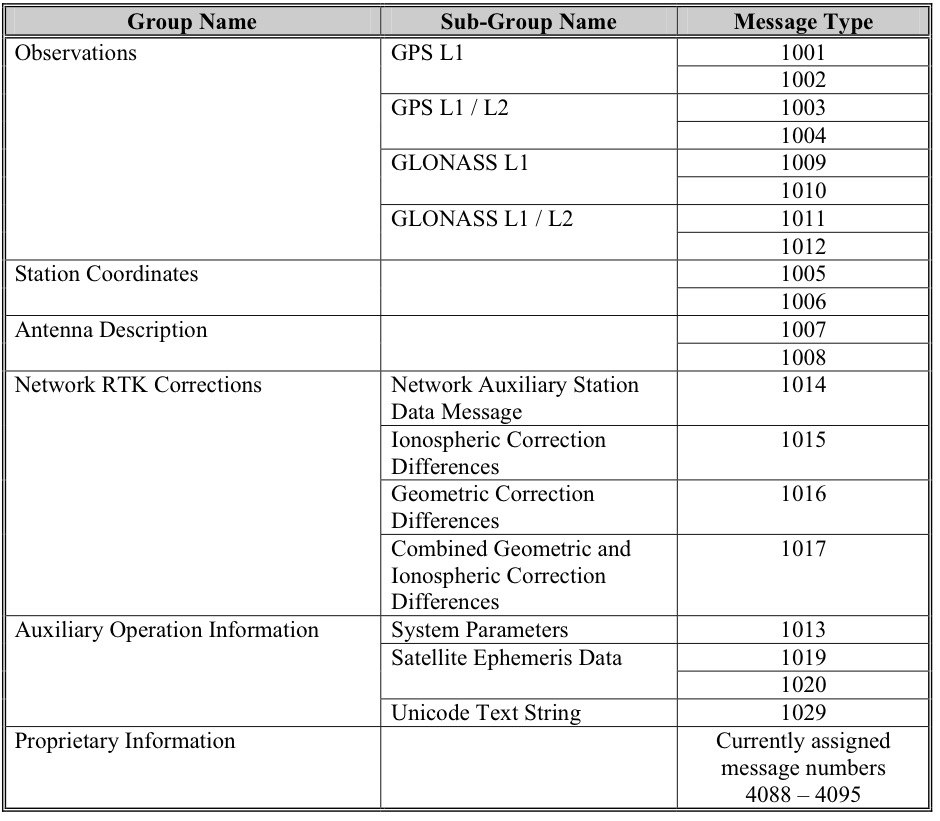
\includegraphics[width=0.7\linewidth]{rtcm_groups.jpg}}
\caption{Группы сообщений в RTCM.}
\label{rtcm_groups}
\end{figure}

Как сказано в \cite{rtcm}, любая система должна поддерживать минимум одно сообщения из каждой группы. Информацию о назначении сообщений, а 
также об их структуре, можно найти в \cite{rtcm}. \par
Ntrip (Networked Transport of RTCM via Internet Protocol) - протокол передачи данных внутри системы дифференциальной навигации. Он описывает 
обмен данными по сети Интернет и построен поверх повсеместно использующегося HTTP/1.1 с добавлением дополнительного типа сообщений. В первую 
очередь предполагается использование протокола для передачи RTCM-поправок, но возможно использовать и иные типы данных. Ntrip реализован в 
виде трех программ: клиента (NtripClient), сервера (NtripServer) и кастера (NtripCaster). Первые два являются HTTP клиентами, тогда как 
последний  - HTTP сервером. Также в Ntrip входит еще один компонент - NtripSource. \\

\begin{figure}[h]
\center{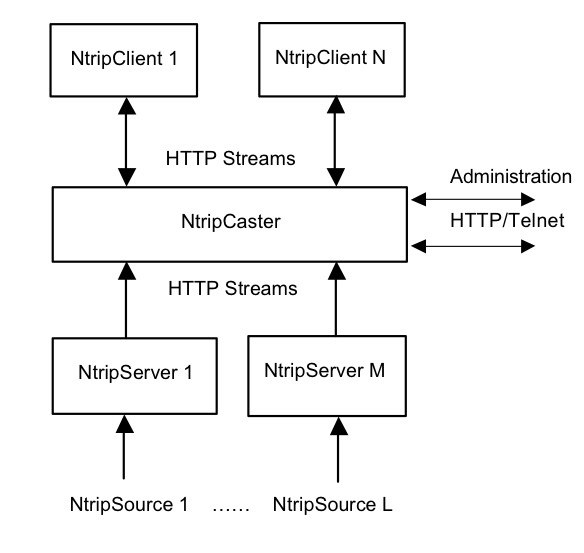
\includegraphics[width=0.7\linewidth]{ntrip.jpg}}
\caption{Схема взаимодействия компонентов в Ntrip.}
\label{ntrip}
\end{figure}

В качестве NtripSource выступает стационарный ГНСС приемник - базовая станция. На ней происходит непрерывный сбор навигационных данных, которые 
затем поступают на NtripServer. Там из них формируется поток, который передается на главный компонент системы - NtripCaster. Затем эти данные 
становятся доступны различным конечным пользователям (NtripClients). На Сервере для каждого связанного с ним Источника вводится специальный 
идентификатор, который называется mountpoint. Различные Клиенты могут получить доступ к данным Источника, запросив их по mountpoint у Кастера. 
У пользователей всегда есть возможность выбрать Источник, с которого они будут получать данные. Для этой цели в Кастере реализована таблица 
источников (source-table). Каждая запись в ней содержит различные параметры потока данных от Источника, такие как mountpoint, координаты 
станции, формат, навигационная система, и т.д. Эти параметры задаются для каждого Источника на Сервере, с которым тот связан. Если клиент, 
запрашивая данные, посылает на Кастер неправильное значение mountpoint или не посылает его вовсе, то вместе ГНСС данных Кастер шлет в ответе 
актуальную таблицу источников, благодаря чему Клиент может сформировать новый запрос. Администратор, ответственный за Кастер, может позволять 
Серверам подключаться с новыми Источниками. Перед тем, как посылать данные, Сервер должен отправить запрос на Кастер, в котором будет указан 
mountpoint и пароль. Оба эти параметра определяются администратором Кастера и заранее передаются администратору Сервера, например посредством 
электронной почты. Клиент, желающий получить данные с Кастера, в запросе должен указать mountpoint и, если того требуют настройки Источника, 
логин-пароль в зашифрованном виде для получения доступа к данным. Если mountpoint указан верно и Клиент проходит аутентификацию, начинается 
трансляция поправок в режиме реального времени. Некоторые Кастеры также имеют возможность хранить полученные от Источников данные для того, 
чтобы Клиенты могли ими воспользоваться для постобработки. Как правило для этого используется ftp-сервер, к которому может подключиться любой 
желающий. Там данные хранятся таким образом, чтобы можно легко получить поправки от желаемой станции на желаемую дату. Чаще всего данные 
хранятся в распространенном формате RINEX.
Среди преимуществ данного протокола можно отметить: \\
- Он основан на популярном стандарте HTTP, что делает его простым в реализации и использовании; \\
- Независимость от типа данных: можно передавать ГНСС данные любого формата; \\ 
- Массовость: возможность одновременной передачи поправок множеству пользователей (с использованием технологии Интернет радио); \\
- Обеспечение безопасности: поставщик и приемник поправок часто не вступают в контакт друг с другом. Поправки не блокируются фаерволом. \\

\newpage

\chapter{Построение сети}
%\addcontentsline{toc}{chapter}{Построение сети}
\section{Примеры}
%\addcontentsline{toc}{section}{Примеры сетей базовых станций}
\par Как уже было отмечено ранее, разнообразие вариантов построения систем дифференциальной навигации велико. Соответственно, существует множество 
уже готовых и функционирующих систем и программных продуктов в этой области. Ниже будут кратко рассмотрены некоторые из них. \par
В первую очередь стоило бы начать с систем SBAS (Satellite-Based Augmentation Systems). Среди них наиболее яркими представителями являются 
уже упомянутые ранее WAAS и СДКМ, а также европейская EGNOS, японская MSAS и индийская GAGAN. Эти широкозонные системы дифференциальной 
коррекции для охвата значительной территории используют космические спутники, которые транслируют поправки пользователям. В этом заключается 
их ключевой недостаток: пользователям указанных сетей необходимо обладать достаточно серьезной аппаратурой, способной принимать сигналы этих 
сетей. В приемники массового производства такая опция не включена. В одно время в СДКМ вводили возможность передачи поправок по сети Интернет. 
В данный момент это используется лишь для режима постобработки; приоритет остается за спутниковым каналом связи. \par
Более удобным и доступным для пользователей вариантом является использование протокола NTRIP. На нем основано множество сетей по всему миру. 
Ниже представлена карта с изображением базовых станций, работающих по NTRIP. Разумеется, на нее нанесены далеко не все.

\begin{figure}[h]
\center{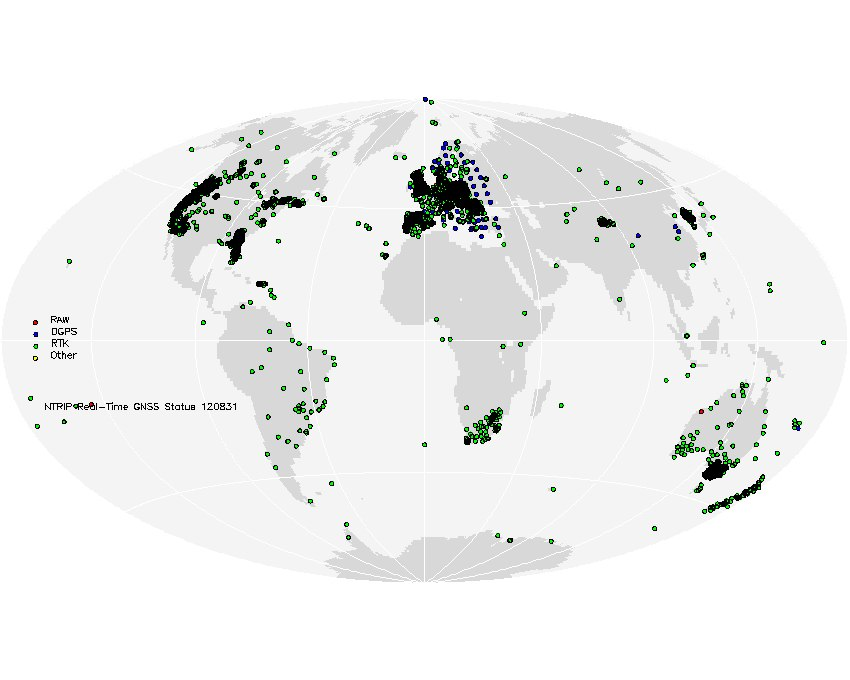
\includegraphics[width=0.9\linewidth]{map.jpg}}
\caption{Распределение базовых станций.}
\label{ntrip}
\end{figure}

Большинство европейских станций принадлежат к сетям IGS (\url{https://www.igs-ip.net/home}) и EUREF (\url{http://www.euref-ip.net/home}). 
На территории Европы эти сети обеспечивают прекрасное покрытие и высокоточные 
результаты. Но в России эти сети представлены лишь одной станцией, которая находится в Звенигороде и принадлежит к IGS. Безусловно, для работы 
на территории России этого недостаточно. \par
В нашей стране также существует ряд различных сетей базовых станций, имеющих различный охват. Наилучшее покрытие обеспечивают Hive GNSS 
(\url{https://hive.geosystems.aero}) и EFT-CORS (\url{http://eft-cors.ru}). Обе в своем составе имеют порядка нескольких сотен станций, 
расположенных преимущественно в европейской части России, и регулярно 
вводят новые. И эти сети были бы идеальными, если бы не одно но: доступ к данным у них платный. Режим RTK у обеих стоит порядка 300 рублей в день. 
Доступ к RINEX файлам у Hive также платный: файлы с интервалом наблюдений в 5 секунд стоят несколько сотен рублей в день, а с интервалом 
в 1 секунду - несколько тысяч. EFT-CORS предоставляет доступ к RINEX бесплатно, но тут же обнаруживается другая проблема: для получения файла 
необходимо заполнить веб-форму. Таким образом, невозможно наладить автоматическую загрузку RINEX файлов. Этой же проблемой обладает и другая 
российская сеть - СВОЭВП (\url{http://www.glonass-svoevp.ru}). Также среди недостатков этой сети можно отметить закрытость информации: 
на сайте не было найдено ничего про базовые станции и используемые технологии. Но она по крайней мере бесплатная. \par
Всеми перечисленными выше недостатками обладает и ряд локальных сетей. На территории Санкт-Петербурга и Ленинградской области это, к примеру, 
Сеть РС СПб (\url{http://ref.kgainfo.spb.ru}) и Геоспайдер (\url{http://geospider.ru}). Стоимость RTK у них может достигать 1000 рублей в день.
\par Таким образом, был выявлен ряд недостатков существующих сетей дифференциальной коррекции, а именно: недоступность массовому пользователю, 
платный доступ к данным, закрытость программного обеспечения и информации о сети, невозможность автоматической загрузки данных. В связи с этим 
было принято решение реализовать собственную сеть, избавленную от перечисленных недостатков.

\section{Реализация NtripServer и NtripCaster}
%\addcontentsline{toc}{section}{Реализация NtripServer и NtripCaster}
\par Сеть сразу было решено делать на основе NTRIP, в связи с достоинствами данного протокола, описанными в предыдущей главе. Для функционирования
NTRIP необходимы базовые станции (NtripSource), кастер (NtripCaster) и программы, обеспечивающие их взаимодействие (NtripServer). Некоторое 
количество станций уже имеется в нашем распоряжении. Среди них: . . . ??? . . . \par
Далее встал вопрос об NtripServer. В большинстве современных дорогих приемников включена поддержка NTRIP. Таким образом, NtripServer встроен 
непосредственно в само оборудование. Но по-прежнему остаются и такие, в которых эта возможность не реализована. Для этого случая требуется 
использовать персональный компьютер: данные с приемников передаются на компьютер, на котором формируются сообщения, содержащие поправки. 
Далее эти сообщения передаются с компьютера на кастер. Некоторые ГНСС приемники используют специальные протоколы для "общения" с компьютерами. 
Среди них оборудование фирм Leica, Trimble и других. Данные фирмы разрабатывают собственные протоколы и продают программное обеспечение, 
способное с ними работать. Но к счастью также существует общепринятый открытый протокол SIRF, реализованный во многих устройствах. \par
Именно на основе этого протокола мною была написана программа, выполняющая функции NtripServer. Она подключается к ГНСС приемнику через 
COM-порт и начинает получать от него навигационные сообщения в формате SiRF. Эти сообщения "на лету" преобразуются в более удобный для чтения 
формат. После того, как устанавливается успешный прием данных с устройства, происходит подлючение к кастеру. Для подключения требуется указать 
специальный пароль и mountpoint. Оба эти параметра должны быть заранее заданы администратором кастера и внесены в соответствующие 
конфигурационные файлы на кастере. После того, как программа получает сообщение о том, что запрос введен правильно, начинается передача 
модифицированных навигационных сообщений. Блок-схема данной программы приведена ниже.

\begin{figure}[h]
\center{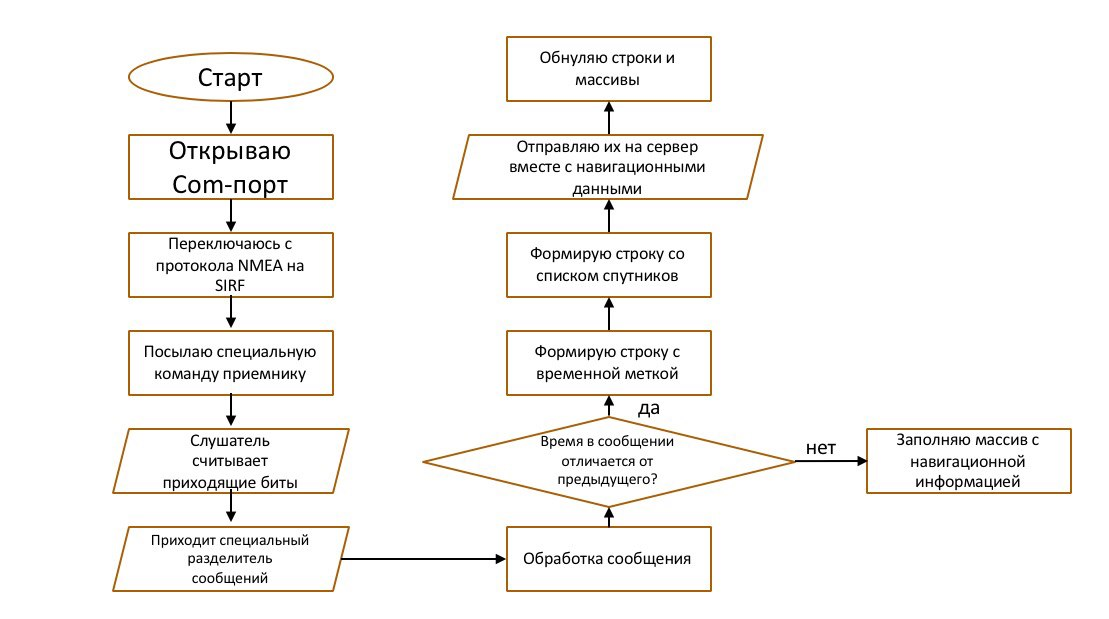
\includegraphics[width=0.9\linewidth]{progr.jpg}}
\caption{Блок-схема реализованного NtripServer.}
\label{ntrip}
\end{figure}

Кастер было решено развернуть на имеющемся в распоряжении кафедры сервере gnss.pu.ru. Изначально планировалось использовать какое-нибудь 
готовое решение. Но оказалось, что большинство существующих кастеров либо платные (например, от BKG - Агентства Геодезии и Картографии, Германия - стоит 
\euro1000), либо не удовлетворяют поставленным требованиям (реализованы под Windows или не 
имеют возможности записи RINEX-файлов). Сводная таблица с найденными кастерами приведена ниже.

\begin{center}
{\footnotesize
\begin{tabular}{| p{4cm} | p{8cm} | p{4cm} |}
\hline
\bf{Название} & \bf{Описание} & \bf{Ссылка} \\ \hline
BKG ntrip caster & Кастер, разработанный немецким Агенством Геодезии и Картографии. Он обладает серьезной функциональностью и используется в 
крупнейших сетях базовых станций, таких как IGS и EUREF. Платный, стоит \euro1000 & \url{https://igs.bkg.bund.de/ntrip/bkgcaster} \\ \hline
Lefebure ntrip caster & Простой в использовании Ntrip кастер. Написан под Windows, бесплатный. Обладает несколько урезанной функциональностью, 
например, не способен сохранять RINEX файлы. Устарел & \url{http://lefebure.com/software/ntripcaster} \\ \hline
SNIP & Недавно разработанный кастер. На данный момент имеется версия под Windows и тестируется ваерсия под Ubuntu. Доступен в трех вариантах: 
Lite (free), Basic (\$495), Pro (\$2495). Указанные варианты отличаются по функциональности & \url{https://use-snip.com} \\ \hline
Standard Ntrip Broadcaster & Open-source кастер, написанный под Linux на языке С. Не имеет интерфейса, работа осуществляется в командной строке. 
Не способен сохранять RINEX файлы & \url{https://github.com/nunojpg/ntripcaster} \\ 
\hline
\end{tabular}
}
\end{center}

На данный момент используется последний кастер из таблицы. Для записи RINEX файлов на ftp-сервер 
используется программа rtcm3torinex, реализованная упомянутым выше BKG. В будущем планируется объединить две эти программы, так как они
обе находятся в открытом доступе. К кастеру успешно подключена станция в Агалатово. Данные в формате RTCM передаются на gnss.pu.ru, 
где они становятся доступными как в формате RINEX, так и в режиме реального времени.

\newpage

\chapter{Применение}
%\addcontentsline{toc}{chapter}{Применение}
\section{Общее описание задачи}
%\addcontentsline{toc}{section}{Общее описание задачи}
\section{Результат использования сети базовых станций}
%\addcontentsline{toc}{section}{Результат использования сети базовых станций}

\newpage

\chapter*{Заключение}
\addcontentsline{toc}{chapter}{Заключение}

\newpage
\addcontentsline{toc}{chapter}{Литература}
\begin{thebibliography}{9}

\bibitem{karut}
	С.Н.Карутин, И.Б.Власов, В.В.Дворкин, 
	\emph{Дифференциальная коррекция и мониторинг глобальных навигационных спутниковых систем}.
	Издательство Московского Университета, Москва,
	2014.
	
\bibitem{kaplan06}
    E. Kaplan, C. Hegarty,
    \emph{Understanding GPS: principles and applications}.
    Artech House, Massachusetts,
    2nd edition,
    2006.

\bibitem{karut-stat}
	С.Н.Карутин,
	\emph{Высокоточное местоопределение по сигналам глобально навигационной спутниковой системы с использованием уточненной эфемеридно-
	временной информации}.
	Вестник МГТУ им. Н.Э.Баумана, Москва,
	2010.

\bibitem{ppp-rtk}
	G.W\"{u}bbena, M.Schmitz, A.Bagge,
	\emph{PPP-RTK: Precise Point Positioning Using State-Space Representation in RTK Networks}.
	2005.

\bibitem{balt}
	В.Л.Горшков, А.В.Мохнаткин, С.С.Смирнов, С.Д.Петров, Д.А.Трофимов, Н.В.Щербакова, 
    \emph{Исследование геодинамики зоны сопряжения Балтийского щита с Восточно-Европейской платформой по данным ГНСС-наблюдений}.
	Вестник СПбГУ, Санкт-Петербург,
    2015.

\bibitem{ntrip}
	H.Gebhard, G.Weber,
	\emph{Ntrip, Version 1.0. Design-Protocol-Software}.
	Federal Agency for Cartography and Geodesy, Frankfurt,
	2003.

\bibitem{rtcm}
	RTCM Special Committee No.104,
	\emph{RTCM Standard 10403.1 for Differential GNSS Services - Version 3}.
	2006.

\bibitem{sirf}
	SiRF Technology, Inc,
	\emph{SiRF Binar Protocol Reference Manual}.
	2008.


\end{thebibliography}

\end{document}
